\documentclass[12pt, a4paper]{scrartcl}
\usepackage[a4paper, left=3cm, right=2cm, top=2cm, bottom=2cm]{geometry}
\usepackage[utf8]{inputenc}
\usepackage[ngerman]{babel}
\usepackage[backend=biber, style=numeric]{biblatex}
\usepackage{tikz} % for drawing
\usetikzlibrary{er, positioning, backgrounds}
\usepackage[linktoc=all, colorlinks, urlcolor=blue, linkcolor=black]{hyperref} % make toc clickable
\usepackage{setspace, graphicx, acronym, csquotes} % minted, subfig für code über mehrere Seiten

\onehalfspacing
\addbibresource{lit.bib}

\sloppy
\setlength{\parindent}{0cm}

\newcommand{\ford}[2]{\textbf{/#1/\hspace{2em}#2}}

\begin{document}
\begin{titlepage}
	\centering
	Berufsakademie Sachsen\\
	Staatliche Studienakademie Leipzig\\
	\vspace{4\baselineskip}
	{\large\textbf{Pflichtenheft}}\\
	\vspace{1\baselineskip}
	{\Large{Campus-Dual Alternative}}\\
	\vfill
	\raggedleft
	\begin{tabbing}
		Seminargruppe:\hspace{2cm}\= 5CS19-1\\[1cm]
		Autoren:\>Max Hohlfeld\+\\
		Martin Junghans\-\\[1cm]
		Version:\>1.0\\[2cm]
		Vorzulegende Stelle:\>Prof. Dr.-Ing. Christian Heller\+\\
		Berufsakademie Sachsen\\
		Staatliche Studienakademie Sachsen\\
		Schönauer Straße 113 a\\
		04207 Leipzig\-\\[2cm]
		Leipzig, den 29.10.2021
	\end{tabbing}
\end{titlepage}

\tableofcontents
\newpage

\section*{Versionsverzeichnis}
\begin{center}
\begin{tabular}{ |p{1.3cm}|p{1.8cm}|p{4cm}|p{6cm}| } 
 \hline
	Version & Datum 	& Autor 				& Kommentar \\\hline
	0.1	& 20.10.2021	& Max Hohlfeld				& Grundgerüst erstellt \\\hline
	0.4	& 25.10.2021	& Max Hohlfeld\newline Martin Junghans	& Aufnahme aller Anforderungen \\\hline
	0.6	& 27.10.2021	& Max Hohlfeld\newline Martin Junghans	& Beschreibung aller Anforderungen \\\hline
	0.8	& 28.10.2021	& Max Hohlfeld\newline Martin Junghans	& Einfügen von Diagrammen \\\hline
	1.0	& 29.10.2021	& Max Hohlfeld\newline Martin Junghans	& Finale Korrekturen und Ergän\-zungen \\\hline
\end{tabular}
\end{center}
\newpage

\section{Einleitung}
\subsection{Grundlage}
Wie bereits im Lastenheft dargelegt, versucht die zu entwickelnde Software die Studentenorganisations-Anwendung Campus-Dual zu ersetzen. Die Erfahrung mit dieser machte eine Entwicklung einer neuen Software sehr interessant. Folge dessen sollen keine Funktionen verloren gehen, sondern viel mehr ein Frühlingsputz der alten Anwendung mit Ergänzung einiger nützlicher Werkzeuge vollzogen werden.

\subsection{Ansprechpartner}
\begin{center}
\begin{tabular}{ |p{7cm}|p{7cm}| } 
 \hline
 Auftraggeber & Auftragnehmer \\\hline
 Prof. Dr.-Ing. Christian Heller\newline
 Berufsakademie Sachsen\newline
 Staatliche Studienakademie Leipzig\newline
 Schönauer Straße 113 a\newline
 04207 Leipzig\newline
 fon: +49-341-42743-415\newline
 fax: +49-341-42743-331\newline
	\href{mailto:christian.heller@ba-leipzig.de}{christian.heller@ba-leipzig.de} &
 Max Hohlfeld\newline
 E-Mail: \href{mailto:s5001554@ba-sachsen.de}{s5001554@ba-sachsen.de}\newline\newline
 Martin Junghans\newline
 E-Mail: \href{mailto:s5001725@ba-sachsen.de}{s5001725@ba-sachsen.de} \\\hline
\end{tabular}
\end{center}
\newpage

\section{Visionen und Ziele}
\ford{Z10}{Ersatz von Campus-Dual}
\begin{itemize}
	\item Erfüllung gleicher Anforderungen
	\item Bereitstellen gleicher Funktionalität
\end{itemize}

\ford{V10}{Fortwährende Nutzung und Weiterentwicklung}
\begin{itemize}
	\item Software ist so attraktiv, dass sie fortwährend genutzt und weiterentwickelt wird
\end{itemize}

\ford{V20}{Revolution in Studentenorganisation der Berufsakademie Sachsen}
\begin{itemize}
	\item Jeder Standort setzt diese Software ein
	\item Jeder Standort macht Anpassungen und Weiterentwicklungen
	\item Berufsakademie Sachsen ist unabhängig von fremder Software
	\item Berufsakademie Sachsen setzt quelloffene Software ein
\end{itemize}
\newpage

\section{Rahmenbedingungen}
\ford{R10}{Anwendungsbereich}
\begin{itemize}
	\item Die Anwendung wird im Rahmen der Studentenorganisation an der BA Leipzig eingesetzt
\end{itemize}

\ford{R20}{Zielgruppe}
\begin{itemize}
	\item Studenten
	\item Dozenten
	\item Organisatoren
\end{itemize}

\ford{R30}{Softwareseitige Anforderungen an den Server}
\begin{itemize}
	\item beliebige moderne Linux-Distribution
	\item Python 3.9
	\item MariaDB 10.3
	\item OpenVPN 2.5 (nur wenn Server außerhalb der DSSAX-Domäne steht)
	\item cifs-utils 6.8
	\item Apache2 2.4 oder nginx 1.14 jeweils mit Unterstützung von WSGI
\end{itemize}

\ford{R31}{Hardwareseitige Anforderungen an den Server}
\begin{itemize}
	\item moderner Prozessor mit mindestens 2 physischen Kernen
	\item 2 GB Arbeitsspeicher
	\item 100 GB Nicht-Flüchtiger Speicher (je nach Menge der Daten irgendwann mehr)
	\item Netzwerkverbindung
\end{itemize}

\ford{R40}{Softwareseitige Anforderungen an den Client}
\begin{itemize}
	\item beliebiges modernes Betriebssystem wie Microsoft Windows, MacOS, Linux-Distribution, Android oder iOS
	\item aktuelle Version von modernen Browsern wie Firefox, Chromium, Safari oder Opera
\end{itemize}

\ford{R41}{Hardwareseitige Anforderungen an den Client}
\begin{itemize}
	\item Beliebiges modernes Gerät mit Internetfähigkeit
\end{itemize}
\newpage

\section{Funktionale Anforderungen}
\ford{F10}{Anzeige bestehender Nutzer}
\begin{itemize}
	\item Darstellung in Tabellenform
\end{itemize}

\ford{F11}{Suche nach Nutzern über Vor- und Nachname oder E-Mail}
\begin{itemize}
	\item Anzeige einer Schaltfläche mit Lupen-Symbol bei den betreffenden Spalten
	\item Bei Klick auf diese öffnet sich ein Eingabefeld
	\item Bei Eingabe wird die betreffende Spalte mit jedem Tastendruck durchsucht
	\item Die Tabelleneinträge werden reduziert auf Einträge, welche der Suche entsprechen
	\item Es gibt einen Knopf, um die Suche zurückzusetzen
\end{itemize}

\ford{F12}{Filtern von Nutzern mittels Seminargruppe}
\begin{itemize}
	\item In Tabellenspalte "`Seminargruppe "' befindet sich eine Schaltfläche mit Filter-Symbol
	\item Bei Klick auf diese wird ein Auswahlfeld angezeigt
	\item Als Auswahlmöglichkeiten gibt es alle vorhandenen Seminargruppen
	\item Nach Auswahl werden nur noch Einträge mit der ausgewählten Seminargruppe angezeigt
	\item Es gibt einen Knopf, um den Filter zurückzusetzen
\end{itemize}

\ford{F20}{Anlegen eines Nutzers}
\begin{itemize}
	\item Erstellen eines neuen Nutzers möglich
	\item Auswahl einer Rolle (Student, Dozent oder Organisator)
	\item Je nach Rolle Forderung unterschiedlicher Mindestangaben
\end{itemize}

\ford{F21}{Bearbeiten eines Nutzers}
\begin{itemize}
	\item Nutzerinformationen können nachträglich verändert werden
\end{itemize}

\ford{F22}{Löschen eines Nutzers}
\begin{itemize}
	\item Nutzer können gelöscht werden
\end{itemize}

\newpage
\ford{F30}{Rolleneinschränkungen}
\begin{itemize}
	\item Studenten und Dozenten besitzen größtenteils nur Lesezugriff
	\item Studenten und Dozenten erhalten nur Zugriff auf die für sie freigeschalteten Objekte
	\item Organisatoren sind Administratoren und erstellen bzw. bearbeiten alle Entitäten
\end{itemize}

\ford{F40}{Passwort-Vergessen-Funktionalität}
\begin{itemize}
	\item Bei der Anmeldung gibt es eine Schaltfläche "Passwort vergessen"
	\item Bei Klick darauf wird dem Nutzer ein Eingabefeld gezeigt, bei welchem er seine E-Mail angeben kann
	\item Daraufhin wird eine E-Mail an die angegebene Adresse geschickt, in welcher ein Link zur Passwort-Zurücksetzen Seite drin ist
	\item Auf dieser Seite kann der Nutzer nach zweifacher Eingabe ein neues Passwort setzen
	\item Dieser Link existiert nur für eine bestimmte Zeit
\end{itemize}

\ford{F50}{Geschützter Bereich nur durch Anmeldung einsehbar}
\begin{itemize}
	\item Die gesamte Anwendung und die beschriebenen Funktionen sind nur nach einer Anmeldung einsehbar
	\item Lediglich öffentlich zugänglich ist eine Startseite mit allgemeinen Informationen über die Anwendung 
\end{itemize}

\ford{F100}{Anzeige existierender Prüfungen}
\begin{itemize}
	\item Tabellenansicht
	\item Anzeige aller eingeschriebenen und angebotenen Prüfungen für jeden Studenten an sich
	\item Anzeige aller Prüfungen eines Dozenten für diesen Dozenten
	\item Anzeige aller Prüfungen für die Organisatoren
\end{itemize}

\ford{F101}{Filtern von Prüfungen nach vergangen und bevorstehend}
\begin{itemize}
	\item In der Tabellenspalte des Prüfungsdatums lässt sich einstellen, ob nur vergangene oder nur bevorstehende Daten angezeigt werden sollen
\end{itemize}

\ford{F110}{Prüfungen anlegen}
\begin{itemize}
	\item Zur Erstellung werden Modul, Start- bzw Enddatum, Raum, Art, Sichtbarkeitsdatum und Fristen zur Einschreibung bzw. Abmeldung
\end{itemize}

\ford{F111}{Prüfungen bearbeiten}
\begin{itemize}
	\item Bestehende Prüfungen sollen auch bearbeitet werden können
\end{itemize}

\ford{F112}{Prüfungen löschen}
\begin{itemize}
	\item Bestehende Prüfungen sollen auch gelöscht werden können
	\item Eingeschriebene Studenten erhalten eine Benachrichtigung darüber und werden von der Prüfung abgemeldet
	\item Bereits vergangene Prüfungen können nicht mehr gelöscht werden
\end{itemize}

\ford{F130}{Prüfungen den Studenten anbieten}
\begin{itemize}
	\item Erstellte Prüfungen werden bestimmten Studenten zur Einschreibung angeboten
	\item Die Prüfung wird für eine bestimmte Seminargruppe erstellt, diese erhält auch das Prüfungsangebot
	\item Alle höheren Semester welche diese Prüfung noch nicht abgeschlossen haben, erhalten ebenfalls dieses Angebot
\end{itemize}

\ford{F131}{Prüfungsangebote ab bestimmen Datum sichtbar schalten}
\begin{itemize}
	\item Die Prüfungsangebote werden ab einem bestimmten Datum sichtbar und lassen sich einschreiben
\end{itemize}

\ford{F132}{Benachrichtigung von Studenten wenn Prüfungsangebote existieren}
\begin{itemize}
	\item Wird ein Prüfungsangebot für einen Studenten sichtbar, so erhält dieser eine Benachrichtigung 
	\item Es herrscht eine gewisse Karenzzeit bevor benachrichtigt wird, sodass möglichst nur eine Benachrichtigung für viele Prüfungen erfolgt 
\end{itemize}

\ford{F140}{Einschreiben in Prüfungsangebote}
\begin{itemize}
	\item Der Student kann sich zur Prüfung anmelden
	\item Organisatoren können Studenten auch zur Prüfung anmelden
	\item Eine Anmeldung führt zur E-Mail an den Studenten als Bestätigung
\end{itemize}

\ford{F141}{Anzeige von eingeschriebenen Prüfungen im Stundenplan}
\begin{itemize}
	\item Der Student sieht, zu welchen Prüfungen er sich bereits angemeldet hat
	\item Der Dozent und Organisator sehen, welche Studenten einer Seminargruppe sich bereits zur Prüfung angemeldet haben
\end{itemize}

\ford{F142}{Berücksichtigen der maximalen drei Prüfungsversuche und damit verbundener Anforderungen}
\begin{itemize}
	\item Nicht erfolgreiche Prüfungen müssen bei der Anmeldung berücksichtigt werden
	\item Zur ersten Wiederholung kann sich Student selber anmelden
	\item Zur zweiten Wiederholung muss ein Antrag ausgefüllt werden; Anmeldung erfolgt also über Organisator 
\end{itemize}

\ford{F150}{Abmelden von eingeschriebenen Prüfungsangeboten}
\begin{itemize}
	\item Der Student kann sich bis zur Abmeldefrist von der Prüfung abmelden
	\item Organisatoren können Studenten auch von Prüfungen abmelden
	\item Eine Abmeldung führt zur E-Mail an den Studenten als Bestätigung
\end{itemize}

\ford{F160}{Abgabe von Hausarbeiten}
\begin{itemize}
	\item Ist die Prüfung keine Klausur sondern eine Hausarbeit, so soll es möglich sein, die Hausarbeit über die Anwendung abzugeben
	\item Bis zu Abgabefrist sollen PDF und ZIP Dateien hochgeladen werden können
	\item Vor Abgabefrist können die Dateien beliebig oft gelöscht oder geändert werden
\end{itemize}

\ford{F161}{Benachrichtigung von Studenten bei gewisser Zeit vor Abgabefrist wenn noch nichts abgegeben wurde}
\begin{itemize}
	\item Wenn ein Student einen Tag vor Abgabefrist noch nichts hochgeladen hat, soll er benachrichtigt werden
\end{itemize}

\ford{F162}{Abruf von abgegebenen Hausarbeiten}
\begin{itemize}
	\item Studenten sollen ihre abgegebenen Dateien auch erneut herunterladen können, um die Korrektheit zu verifizieren
	\item Dozenten sollen die Arbeiten gesammelt sowie je Student herunterladen können
\end{itemize}

\ford{F170}{Eintragen von Benotungen}
\begin{itemize}
	\item Dem Dozent und dem Organisator ist es möglich, für eine Prüfung eines Studenten eine Note einzutragen
	\item Die Benotung führt zu einer Benachrichtigung des Studenten
\end{itemize}

\ford{F171}{Ansicht der Note einer Prüfung}
\begin{itemize}
	\item Der Student kann sich seine Note einer Prüfung anzeigen lassen
\end{itemize}

\ford{F172}{Darstellung einer Statistik über alle Ergebnisse einer Prüfung}
\begin{itemize}
	\item Student und Dozent können zu jeder erfolgten und vollständig benoteten Prüfung eine Statistik einsehen
	\item Die Ausweisung der Noten erfolgt anonymisiert als Balkendiagramm
\end{itemize}

\ford{F200}{Erstellen von Ereignissen für bestimmte Seminargruppen}
\begin{itemize}
	\item Es lassen sich Ereignisse erstellen
	\item Dazu werden Start- bzw. Enddatum, Raum, Seminargruppe und das dazugehörige Modul benötigt
\end{itemize}

\ford{F201}{Bearbeiten von Ereignissen}
\begin{itemize}
	\item Erstellte Ereignisse können auch bearbeitet werden
\end{itemize}

\ford{F202}{Löschen von Ereignissen}
\begin{itemize}
	\item Erstellte Ereignisse lassen sich auch löschen
\end{itemize}

\ford{F210}{Stundenplanansicht}
\begin{itemize}
	\item Student sieht den Plan für seine Seminargruppe sowie die personalisierten Prüfungsangebote
	\item Dozent sieht Plan mit den ihn betreffenden Ereignissen(Vorlesung, Prüfung)
	\item Organisator kann auswählen, welcher Plan angezeigt werden soll (Auswahl nach Seminargruppe oder Dozent)
\end{itemize}

\ford{F211}{Unterschiedliche Darstellung von Prüfungen und Vorlesungen in der Ansicht}
\begin{itemize}
	\item Prüfungen werden rot hinterlegt angezeigt
	\item Vorlesungen werden orange hinterlegt angezeigt
\end{itemize}

\ford{F212}{Vor- und Zurückblättern in Stundenplanansicht}
\begin{itemize}
	\item Anzeige von zwei Schaltflächen bei der Stundenplanansicht (vor und zurück)
	\item Bei Klick wird die jeweils vorangegangene bzw. folgende Zeitdauer in der Ansicht dargestellt
\end{itemize}

\newpage
\ford{F213}{Darstellung zwischen Monat(Standard), Woche und Tag wechselbar}
\begin{itemize}
	\item Die Feinheit der Darstellung kann verändert werden
	\item Standardmäßig wird immer ein Monat dargestellt
	\item Es sollen sich aber auch nur einzelne Wochen oder Tage darstellen lassen
\end{itemize}

\ford{F220}{Stundenplan exportierbar im iCalendar-Format}
\begin{itemize}
	\item Der Student kann sich seinen Stundenplan als Kalenderdatei im iCalendar-Format ausgeben lassen
\end{itemize}

\ford{F300}{Generierung von offiziellen Dokumenten}
\begin{itemize}
	\item Dazu zählen Notenbescheinigung, Immatrikulationsbescheinigung und BAföG-Dokumente
\end{itemize}

\ford{F301}{Anzeige dieser Dokumente im Browser}
\begin{itemize}
	\item Anzeige mittels Einbettung des Browser-internen PDF-Viewers
\end{itemize}

\ford{F302}{Export dieser Dokumente als PDF}
\begin{itemize}
	\item Schaltfläche zum Exportieren anzeigen
	\item Bei Klick wir das Dokument als PDF heruntergeladen
\end{itemize}

\ford{F400}{Anzeige von Inhalt auf dem Fileserv}
\begin{itemize}
	\item Anzeige eines File-Browsers im Internet-Browser
	\item Navigation analog zum Betriebssystem-eigenen File-Browsers
\end{itemize}

\ford{F401}{Download von Inhalten vom Fileserv}
\begin{itemize}
	\item Bei Klick auf Datei im File-Browser wird diese heruntergeladen
	\item Bei Rechtsklick auf Ordner lässt sich dieser auch als ZIP-Archiv gepackt herunterladen
\end{itemize}
\newpage

\section{Qualitätsanforderungen}

\ford{QEZ10}{Qualitätsanforderung nach Effizienz(Zeitverhalten)}
\begin{itemize}
	\item Software soll so wenig externe Bibliotheken einbinden wie möglich
	\item Software soll schnell sein
\end{itemize}

\ford{QBE10}{Qualitätsanforderung nach Benutzbarkeit(Erlernbarkeit)}
\begin{itemize}
	\item Menüführung soll einfach sein
	\item Schaltflächen sollen das tun, was der Nutzer erwartet
\end{itemize}

\ford{QBA10}{Qualitätsanforderung nach Benutzbarkeit(Attraktivität)}
\begin{itemize}
	\item Benutzeroberfläche soll sauber und ansprechend gestaltet sein
\end{itemize}

\ford{QBA10}{Qualitätsanforderung nach Benutzbarkeit(Bedienbarkeit)}
\begin{itemize}
	\item Benutzeroberfläche soll dafür sorgen, dass die Bedienung so leicht wie möglich ist
\end{itemize}

\ford{QFS10}{Qualitätsanforderung nach Funktionalität(Sicherheit)}
\begin{itemize}
	\item Die gespeicherten Daten sind personenbezogen und bedürfen besonderes Schutzes
	\item Keine Einbindung externer Skripte oder Stylesheets um eine Aktivitätsverfolgung auszuschließen
\end{itemize}

\ford{QFR10}{Qualitätsanforderung nach Funktionalität(Richtigkeit)}
\begin{itemize}
	\item Es werden wichtige Daten verarbeitet
	\item Diese dürfen auf keinen Fall unselbständig durch die Anwendung verändert werden
\end{itemize}
\newpage

% \section{Abnahmekriterien}

\section{Modelle und Diagramme}
\subsection{Entity-Relationship-Modell}
\begin{figure}[h]
	\centering
	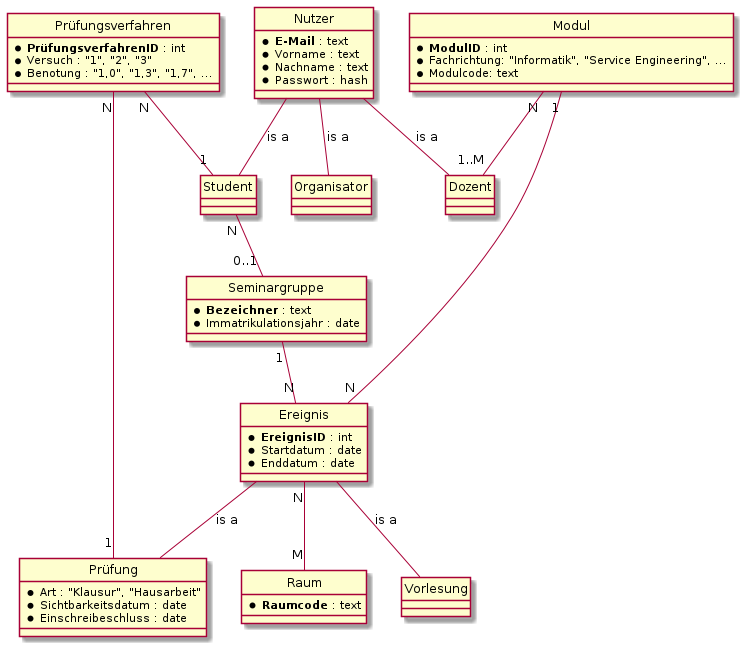
\includegraphics[width=\textwidth]{erm.png}
	\caption{Entity-Relationship-Modell der Campus-Dual-Alternative}
\end{figure}

\newpage
\subsection{Anwendungsfall-Diagramme}
\begin{figure}[h]
	\centering
	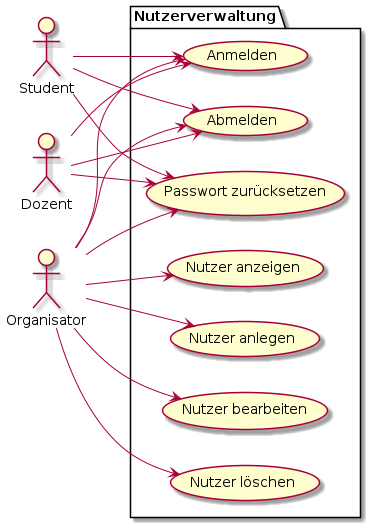
\includegraphics[width=.6\textwidth]{usecase_nv.png}
	\caption{Anwendungsfall-Diagramm Nutzerverwaltung}
\end{figure}

\begin{figure}[h]
	\centering
	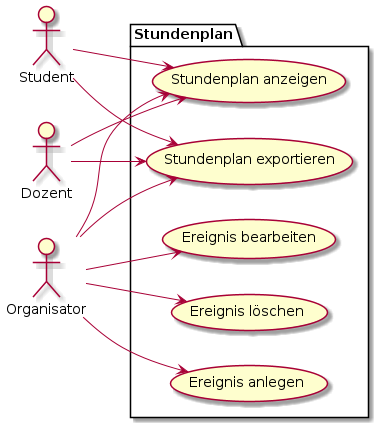
\includegraphics[width=.6\textwidth]{usecase_sp.png}
	\caption{Anwendungsfall-Diagramm Stundenplan}
\end{figure}

\begin{figure}[h]
	\centering
	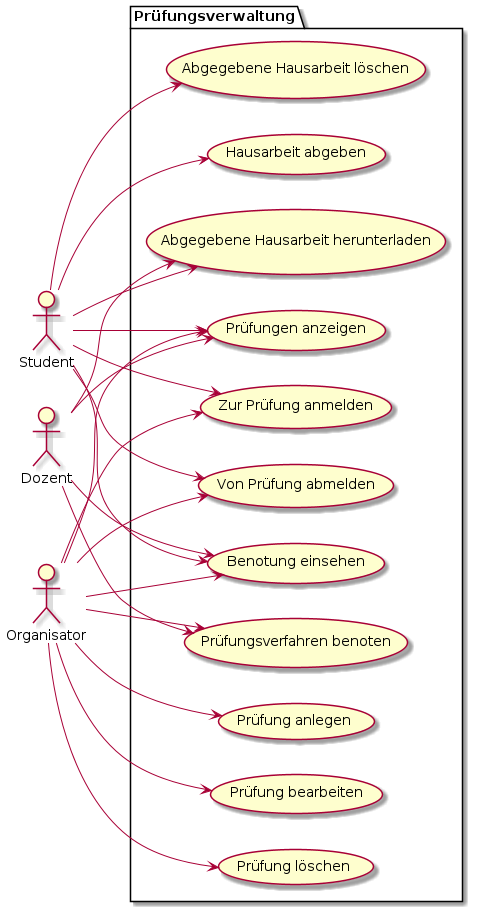
\includegraphics[width=.6\textwidth]{usecase_ex.png}
	\caption{Anwendungsfall-Diagramm Prüfungsverwaltung}
\end{figure}

\begin{figure}[h]
	\centering
	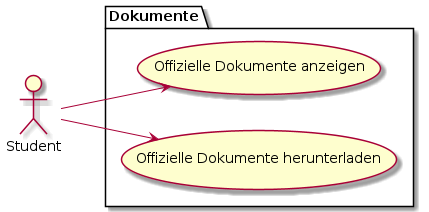
\includegraphics[width=.6\textwidth]{usecase_do.png}
	\caption{Anwendungsfall-Diagramm Dokumente}
\end{figure}

\begin{figure}[h]
	\centering
	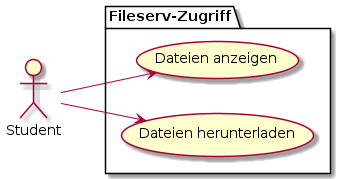
\includegraphics[width=.6\textwidth]{usecase_fs.png}
	\caption{Anwendungsfall-Diagramm Fileserv}
\end{figure}

\end{document}
